% THIS IS AN EXAMPLE DOCUMENT FOR VLDB 2012
% based on ACM SIGPROC-SP.TEX VERSION 2.7
% Modified by  Gerald Weber <gerald@cs.auckland.ac.nz>
% Removed the requirement to include *bbl file in here. (AhmetSacan, Sep2012)
% Fixed the equation on page 3 to prevent line overflow. (AhmetSacan, Sep2012)

\documentclass{vldb}
\usepackage{graphicx}
\usepackage{balance}  % for  \balance command ON LAST PAGE  (only there!)



\begin{document}

% ****************** TITLE ****************************************

\title{Client-Side Indexes for Fast Full-Text Searching}

% possible, but not really needed or used for PVLDB:
%\subtitle{[Extended Abstract]
%\titlenote{A full version of this paper is available as\textit{Author's Guide to Preparing ACM SIG Proceedings Using \LaTeX$2_\epsilon$\ and BibTeX} at \texttt{www.acm.org/eaddress.htm}}}

% ****************** AUTHORS **************************************

\numberofauthors{3}

\author{
\alignauthor
Amy X. Zhang\\
       \email{axz@mit.edu}
\alignauthor Lea Verou\\
       \email{leaverou@mit.edu}
\alignauthor Manali Naik\\
       \email{manalinaik@mit.edu}
}

\maketitle

\begin{abstract}

Many applications on the web use a combination of client-side and server-side data stores to facilitate fast interactive and data-intensive experiences. 
However, standard client side databases within browsers do not currently support full-text searching. 
In this paper, we describe a client-side search engine built on top of IndexedDB that makes use of several types of indexes common to many well-known server-side search engines.
We compare the performance of different indexes on different types of full-text content and queries and find that....
We also compare the performance of our system with that of fully server side systems and examine scenarios where a hybrid approach may be fastest. We find that...

\end{abstract}

\section{Introduction}

Most web applications store the bulk of their data on a backend web server or on the cloud, and the client side queries the server when it needs to access data.
As web applications have become more interactive and responsive in the past several years, developers have built larger and more complex web servers to support them. However, this separation of data from the client introduces significant network effects that can often lead to noticeable latency, as data may be retrieved from servers that are very far away. 

In recent years, more applications are being built that heavily rely on client-side storage and offload data processing to web browsers. Today most commonly used browsers support the current HTML5 standards, which include a persistent client-side DBMS with the name IndexedDB that is accessible via a set of JavaScript APIs. 
The ability to use local storage enables real-time interactivity on data-intensive and collaborative tasks by reducing the number of network roundtrips.
These have been useful for many large and complex web applications such as massive multi-player games CITE that would have previously only existed as desktop applications.
Issues around privacy and ownership of data have also given rise to a number of applications CITE that move most or all of data storage to the client~\cite{bilenko2011predictive}. 
Finally, many popular smartphone browsers rely on wireless signals to transmit information, which is prone to failure in areas with poor signal, suggesting that applications that are entirely client-side or applications that retains some functionality during downtime could be useful~\cite{balasubramanian2012findall}.

While much work has been done to make it easier to store and query data in the browser~\cite{benson2010sync}, currently there are few known ways to conduct full-text searching on the client side. Search engines are a very important component of a large number of applications and are necessary to make sense of many forms of full-text data such as chat or private messages, social media content, search queries, and webpage titles and content. 
As personalization has become more important for search engines, many designers of systems and architectures have highlighted the opportunities for client-side data computation~\cite{bharat2000searchpad,teevan2005personalizing}.
Issues of privacy are also important when it comes to social applications and searching over personal data. New social applications such as CITE have been built that can operate without any servers, instead using peer-to-peer or Bluetooth connections.
However, while it is possible to store full-text content on the client side, there is still no way to conduct full-text search on the client side at a reasonable speed, preventing most data computation necessary for a fully-featured search engine.
The current standard of IndexedDB, a key-value store, only supports simple operations such as put and get on set of keys and secondary indexes on object fields. There are no built-in capabilities to create indexes for full-text content. 

In this paper, we introduce Lucy.js, a fully client-side JavaScript search engine that is an extension of the current IndexedDB API CITE. It has been designed to be easy for anyone currently using IndexedDB in their application to begin indexing and searching full-text content, without needing to modify pre-existing code or move to a new framework or mode of communication. There are also no dependencies on a server or on a network, so it can be harnessed offline. In our implementation, we created several types of indexes commonly used in well-known search engines, such as Lucene CITE and within PostgreSQL CITE, including inverted indexes, prefix and suffix tries, and lossy search trees. We discuss how we managed to create these indexes on top of the IndexedDB framework as well as how the different indexes are suited to different tasks. We compare their performance on different types of queries and with different sizes and types of datasets. We find that...

Finally, we imagine the potential real-world use cases for a client-side search engine and how performance may be improved using this system. We implement a set of applications that would be reasonable in the real world and measure performance between fully client-side, fully server-side, and mixtures of both databases to respond to queries. We find that....
This research demonstrates not only the feasibility of having search engines within the browser but also the potential for new applications and improved performance of existing applications through the additional capabilities provided by a client-side search engine.


\section{Background and Related Work}

Though previous HTML standards and browser capabilities were more limited, the idea of using of the client side for data storage and data computation has been around for many years. 
Some research has looked into building tools to support an architecture that includes client-side databases, including toolkits to synchronize data between the client and server~\cite{benson2010sync}. Another project facilitates ubiquitous access to client-side data across multiple browsers by enabling browser session migration from client to server to client~\cite{lo2013imagen}. 

When it comes to search engines, specifically web search, prior work has found that 40\% to 60\% of search queries are re-finding queries~\cite{teevan2005personalizing}. This finding has lead to applications that store web content from the result of a search engine to improve speed and availability when the network is down~\cite{bozzon2010liquid,bharat2000searchpad,balasubramanian2012findall}. Prior work in this area have also highlighted how web search can often be a highly personal activity, and that web search should be personalized to the user to improve accuracy. Personal information can then be stored on the client side as this information is primarily useful for this particular client~\cite{teevan2005personalizing}.
Privacy is also a large concern for applications that collect personal data. Some applications have tackled personalized advertising using client-side stored profiles to mitigate this problem~\cite{bilenko2011predictive}.

With the increased use of mobile phones in recent years, many web applications are now accessed via a smartphone. Here too, studies have shown that many queries to search engines are for re-finding. Using a client-side database is potentially even more impactful for a mobile phone browser because network connectivity is much less robust. Researchers have demonstrated this feasiblity by building a standalone search application for Android~\cite{balasubramanian2012findall}. However, this search engine is not usable with other browsing apps or other phones. Because we build an extension on top of IndexedDB, our search engine will be able to work for all browsers, desktop or mobile, that support IndexedDB, which is the majority of them.

Some prototypes of client-side search engines have previously been built CITE. Currently, all existing implementations only create basic inverted indexes.
For instance, previous research has demonstrated that it is feasible to store an inverted index within IndexedDB~\cite{lin:jscene} though it is much slower than using a server-side application such as Lucene.
We improve on these works by implementing different types of indexes for full-text search and comparing their performance. 
Another existing implementation of a client side search engine called Lunr.js\footnote{http://www.lunrjs.com} stores indexes in the client-side memory, which is infeasible for large amounts of data and also non-persistent. Instead, our system uses IndexedDB object stores to hold indexes. Also, the YDN-DB module\footnote{https://github.com/yathit/ydn-db-fulltext} which wraps around the IndexedDB API, requires developers to migrate over to use the YDN system. Instead our system is simply an extension of IndexedDB.
We also demonstrate several real-life situations that may call for a hybrid client and server database architecture for full-text search and measure their speed.


\section{Architecture and Overview}

In this section, we explain the overall goals and architecture of the Lucy.js system, how it fits into IndexedDB, as well as give further details of our implementation. 


\begin{figure}[]
   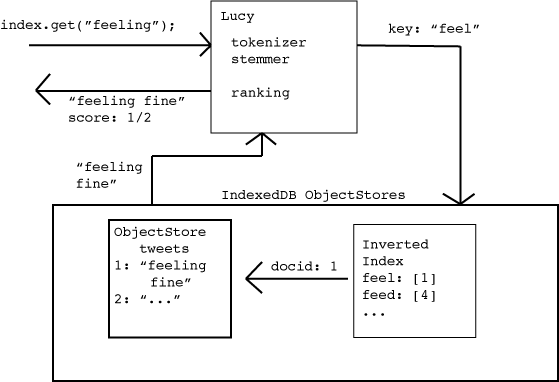
\includegraphics[scale=.43]{arch}
  \caption{caption here.}
\end{figure}

\subsection{Goals}

The two main goals of Lucy.js we aimed to achieve while implementing it were: (i) to build a search engine extension to IndexedDB that is easy to use and similar to the existing IndexedDB API, and (ii) to create different types of indexes that can all be used for full-text searching and find out which are more suited to which tasks and what the trade-offs are. We design Lucy.js so that it is easy as a developer to be able to specify which type of index to make on a field based on the type of queries that will most often be submitted.

\subsection{IndexedDB}

Indexed Database (IndexedDB) is a collection of Javascript APIs and is an official W3C specification (Proposed Recommendation stage) ~\cite{w3c}. It is supported by almost every modern browser, both on desktop and mobile devices. Chrome, Firefox, Internet Explorer, Opera, and Safari are only some of the browsers that have added support for IndexedDB in their modern versions. For our implementation, we focused our testing and demos on the Chrome browser as it is currently the most widely used.
On Chrome browsers, IndexedDB interfaces with a key-value store named LevelDB built at Google in C++ and inspired by BigTable. In LevelDB, keys and values are arbitrary byte arrays and data is stored in sorted order by key. It supports batch writing, put and get commands using the key, and forward and backward iteration over keys. 

The IndexedDB API supports transactions that rely on shared read and exclusive write locking. At transaction creation time, the code must specifies what kind of transaction it is (read-only, write-only, or read-write) and what object stores (similar to tables in a relational data store) it will access.  Read-only transactions can run concurrently but transactions that write lock the specified object stores for the entire duration of the transaction.
All transactions in IndexedDB are asynchronous, meaning that one must request for a database operation, such as a put or a get, to happen and then pass a callback function. Then a notification via a DOM event is triggered when the operation actually completes, and the type of event returned tells whether the operation succeeded or failed.


\subsection{Extending IndexedDB}

\subsubsection{Creating a Full-Text Index}
The interface to a database is maintained through an \texttt{IDBDatabase} object.
To alter the schema of an IndexedDB database, for instance to create a new object store, the code must update the database version from its current version. This is not necessary when creating a normal secondary index on an existing object store. However, it will need to be updated when creating one of our new full-text indexes, as they are stored in IndexedDB as regular object stores. Thus the developer needs to persist locally the current version of the database and increment it before creating a new full-text index. Otherwise, the creation of a full-text index is very similar to that of a normal index. Given the object store \texttt{IDBObjectStore} that the index will be created on, we repurpose the existing \texttt{createIndex$\left(index\_name, key\_path\right)$} function for creating full-text indexes. We add an additional optional parameter of \texttt{type} which allows the developer to specify a type of full-text index they would like to build. The full-text index options we allow are \texttt{inverted}, \texttt{prefix}, and \texttt{suffix}. If the developer does not specify a type, then a typical IndexedDB index would be created. Below is an example of JavaScript code to create an inverted index called \texttt{tweets\_text} on an object field \texttt{text} in an object store of Twitter tweets.

\begin{verbatim}
var newDBVersion = incrementDBVersion();
var DBRequest = indexedDB.open(databaseName,
                               newDBVersion);
DBRequest.onupgradeneeded = function(evt) {
     var tn = evt.target.transaction;	
     var objStore = tn.objectStore("tweets");
     objStore.createIndex("tweets_text", "text", 
                          {"type": "inverted"});
};
DBRequest.onsuccess = function(evt) {
     evt.target.result.close();
};
\end{verbatim}


\subsubsection{Searching over a Full-Text Index}

There are two ways to retrieve items given an \texttt{IDBIndex} object using the IndexedDB API. 
The first is to use a \texttt{get} function, which returns an \texttt{IDBRequest} object with the \texttt{result} field populated with the value in the object store that corresponds to the given index key. The second is to call \texttt{openCursor}, which returns an \texttt{IDBCursor} object that can be iterated over. One can pass in a range of keys instead of just one key to either function, using the \texttt{IDBKeyRange} interface.

In our case, a given search query may return many results that have different levels of relevance to the query. For this reason, each object returned has an addition field called \texttt{score}, which has a relevancy value with higher being more relevant. 
In the next section, we go into more detail into how the score is calculated for different types of search queries.
By default we return all relevant (\texttt{score} $>$ 0) objects in reverse order of \texttt{score}. 

However, a query can return a large number of items with low relevancy if the query contains a term that is common. In IndexedDB, there is an interface called \texttt{IDBKeyRange} that is used for when a user wishes to query a range of keys. We extend this interface to include ranges of \texttt{score} values, so that users can set a cutoff or range of the relevancy score. This feature is also one that is available in PostgreSQL as **********.

In the follow code snippet, we provide an example of a \texttt{get} function on the inverted index created in the last section. The object returned is an \texttt{IDBIndexRequest} object, which mimics the behavior of \texttt{IDBRequest}.

\begin{verbatim}
var index = objStore.index("tweets_text");
var request = index.get("follow friday");
request.onsuccess = function(evt) {
     console.log(request.result);
};
\end{verbatim}

The following is an example of generating a cursor over a query on a full-text index. The cursor can be made to play forwards or backwards over the intended order using the parameter value of \texttt{next} or \texttt{prev}.

\begin{verbatim}
var index = objStore.index("tweets_text");
var request = index.openCursor("#nowplaying", "next");
request.onsuccess = function(evt) {
     var cursor = event.target.result;
     if(cursor) {
          console.log("Text: " + cursor.value.text +
                      "Score:" cursor.value.score);
          cursor.continue();
     }
};
\end{verbatim}

Other functions of \texttt{IDBIndex} that are supported include \texttt{getKey}, which returns the primary keys on the original object store that are the result of a query, and \texttt{count}, which returns the number of relevant objects.


\subsection{Natural Language Processing}

Queries to our full-text search engine can be words or phrases. In addition, they can contain a special wildcard symbol \textbf{\%} at the start or end of any word to search for parts of words. At this time, we do not support full regular expressions nor exact phrase matches.

The processing that we conduct on queries and on the full text is standard for most search engines such as Lucene, MySQL, and PostgreSQL. The first thing we do is tokenize the text into contiguous strings of alphabetic characters, which are generally words. We convert the entire text to lower case and then remove stopwords from the bag of words. The stopword list we employ is taken from MySQL's full-text stopword list\footnote{http://dev.mysql.com/doc/refman/5.1/en/fulltext-stopwords.html}. The reason we remove stopwords is because these words are present in much of natural language and including them could grow the result set to be very large but not return very relevant results.

Next, we employ stemming on each individual word using an open source JavaScript implementation of a Snowball stemmer\footnote{https://github.com/fortnightlabs/snowball-js}. 
Stemming can be a useful part of search engines because a user may be interested in text containing a word even if the word is pluralized or has some other form of suffix.

Sometimes however these processing techniques are not desired, given a particular type of text, type of query, or type of index used. For instance, stemming does not make sense when we are building a suffix trie. Our system allows the developer to pass optional parameters to disable stopword removal or stemming when desired. It is also possible for developers to edit the stopwords list for a list that is domain-specific or otherwise more preferred.

Finally, our system offers flexible support for other languages. The stemmer that we employ has support for 14 common languages in addition to English. When creating an index, a developer can specify as an optional parameter the language the full-text strings are in. Then, when it comes time, the stemmer will choose the given language to use for stemming.
Also, the stopword list is included as a separate JavaScript file. To swap out one language's stopwords with another's, one only needs to replace the JavaScript file imported in the HTML page. This prevents web pages from having to load stopword lists of all supported languages when using Lucy.js. 

\subsection{Scoring and Ranking Results}

There are many ways to score and rank results of a search query. Some techniques, such as \textit{tf-idf}, require constant recalculation of document metadata. Others require knowning positional information about a word within a document. We define several built-in ranking functions derived from PostgreSQL's built-in \texttt{ts\_rank} and \texttt{ts\_rank\_cd} functions that take in a \texttt{normalization} option, with integer inputs providing different types of document normalizations\footnote{http://www.postgresql.org/docs/8.3/static/textsearch-controls.html}.
The PostgreSQL's functions take into account how often the query terms appear in the document as well as how close together the terms are in the document. However, it is possible for a developer to implement their own ranking function and replace ours with theirs within Lucy.js if they so wish.

One function that we provide is \texttt{Lucy.calculateWeight()}, which counts the number of words in the search query that appear in the document. The other ranking we provide is \texttt{Lucy.calculateCoverDensity()}, which implements Cover Density Ranking~\cite{li2002improvement}, an algorithm that takes into account positional information. For this algorithm to work, we need to store at index creation time the positions that the word appears in the document. Both functions take in an optional \texttt{normalization} integer where the developer can specify whether they are interested in normalizing by document length or unique number of words in the document. If normalization is desired, then at index creation time, we calculate these measures and store them with the document object.

\subsection{Implementation}

We created Lucy.js in JavaScript, as the IndexedDB API is also in JavaScript. The code consists of three main files - \texttt{lucy.js}, \texttt{invindex.js}, and \texttt{trieindex.js} that the developer must include in their HTML file. The user should also additionally add one of the \texttt{<language>\_stopwords.js} files in order to pick a language to check stopwords on.

The file \texttt{lucy.js} contains a static class called \texttt{Lucy} which holds various text processing functions that the different indexes use. There is also an extension of \texttt{IDBRequest} called \texttt{IDBIndexRequest} that provides the same behavior, only for our full-text indexes. Finally, there are a set of functions that intercept functions of \texttt{IDBObjectStore}. When a user calls \texttt{create\_index} or \texttt{index}, if they are creating or referring to a full-text index we direct the function to one of our index implementations. When a user calls \texttt{add},  \texttt{delete}, or \texttt{put} on an object store that has a full-text index, we additionally add the item to our indexes.






\section{Index Implementations}

We looked to many existing implementations of search engines and the indexes they used. Reverse indexes in Lucene. GiN and GiST indexes in PostgreSQL. Prefix and suffix tries from 

\subsection{Inverted Indexes}

\subsection{Prefix and Suffix Tries}

Trie indexes are used to perform prefix and suffix searches on text data. While prefix/suffix search is often used for pattern-matching that matches the entire original text, the trie index in Lucy.js uses tokenization to perform finer-grained searches on multi-word text inputs (like tweet data). Phrase search with tries is also supported. This allows users to search by multiple prefixes or suffixes at a time, and get results with the most matches.

Prefix and suffix tries are implemented using the same design. The only difference between them is that words are reversed before insertion into suffix tries, and similarly, search terms are reversed before they are looked up in the suffix trie. Otherwise, they rely on the same implementation as described below.

A trie index in Lucy.js (prefix or suffix trie) is represented by two underlying entities in IndexedDB: an objects store to save nodes in the trie, and an index on that object store to make trie traversal faster.  A reference to the input object store to be indexed -- which contains the full-text to be searched -- is also saved.

\subsubsection{Trie Node Object Store}
Each entry in the object store represents a different node in the trie. The structure of entries in the object store is as follows:
\begin{center}
node\_id: \{ parent\_id: a, char: b, doc\_ids: [x,y,z] \}
\end{center}
The key to the object store is the node\_id, and the corresponding value object has three attributes: parent\_id, char, and doc\_ids. The parent\_id attribute is the node id of the parent node in the trie, and the char attribute is the character value for the trie node. The final attribute is doc\_ids, which is a list of keys into the input text object store. The keys in this list are like foreign keys that allow the trie index to retrieve the actual text from the input object store when answering queries. Each path -- and therefore each node -- in the trie represents a unique prefix/suffix. The doc\_ids for a node contains the ids of all documents with that given prefix/suffix. Inserting a word from a given document therefore involves appending that document's id into the doc\_ids of each node along the path corresponding to the word. The structure of the trie is shown in Figure ******.  It is important to note that this approach is not very scalable; since each node stores a list of matching document ids, interior nodes closer to the root of the trie could store large lists of these ids. However, the benefit is that searches in the trie do not require traversal all the way down to the leaves. Matches can be returned as soon as the prefix is traced in the trie, and no further traversal along subtrees is needed. An alternative design to the trie index is the Hybrid Trie discussed in the next section.

\begin{figure}[h!]
  \centering
   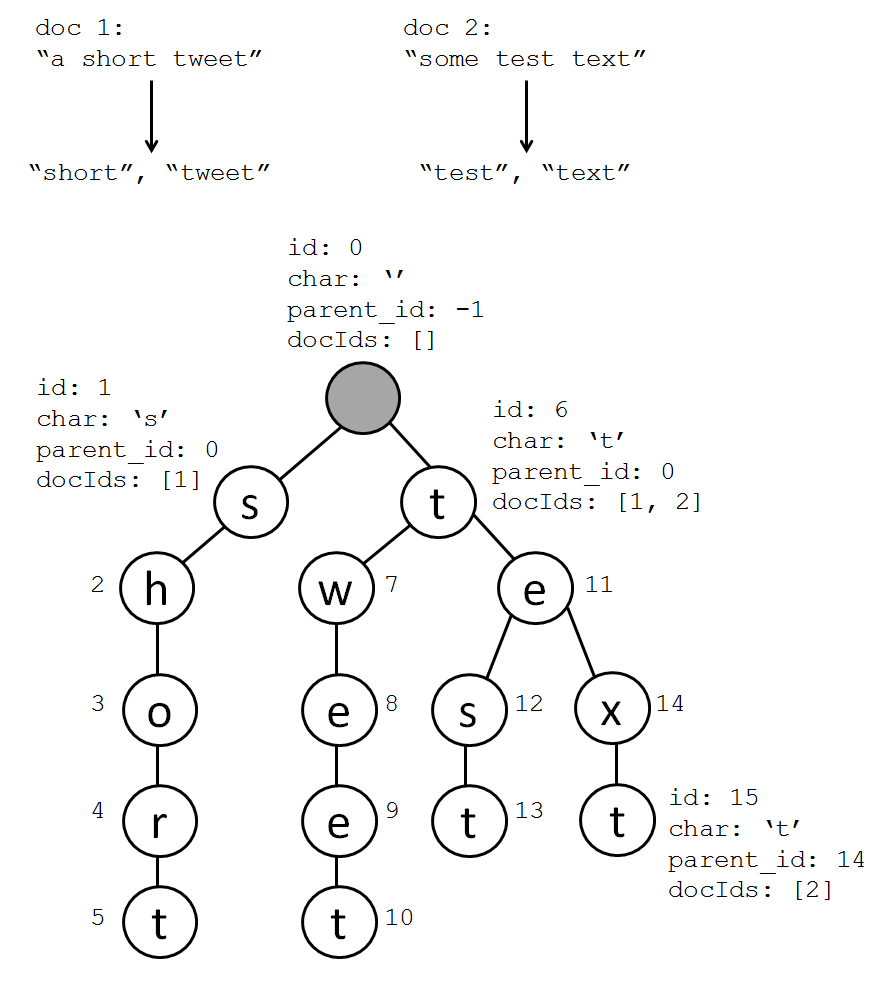
\includegraphics[scale=.35]{trie_figure}
  \caption{Structure of a trie index with two input tweets. The tweets are first tokenized and stop words are removed. Note that document ids are stored in every node. An artificial root node is created as the root of the trie.}
\end{figure}

\subsubsection{Trie Node Index}
While the structure of the trie node object store optimizes lookups by node id, this is not particularly useful for trie traversal. When traversing down a trie, we would instead like to look up nodes by both their character value and their parent id. It would have been possible to change the design of the trie object store so that each node stored a list of children node ids instead of a single parent id. However, this approach requires each node to store more information, since a list of children ids is saved per node instead of a single parent id. Additionally, we would then need to iterate over this list of children ids in order to find a particular child node with a given character value. With the current object store structure, we can optimize lookups by parent\_id and char by building an index on both these attributes. Overall, the trie index is backed by an object store for node storage and an index on that object store with a compound key of both parent\_id and char.

\subsubsection{Lookups}
Lookups in the trie index are performed by traversing the trie downward, character by character in the search pattern. Partial matches are not accepted; the entire prefix (or suffix) must be present in the trie or no results are returned. If the entire pattern is found, the doc\_ids are extracted from the trie node corresponding to the last letter of the search pattern. These ids are used to key into the input text object store and retrieve the original text data.

\subsubsection{Tokenization}
Unlike with the inverted index, words are not stemmed before insertion or lookups. This is especially important for suffix tries because many suffix searches will not succeed due to stemming of the original text being searched. Tokenization is still used to break up input into words; it is used during both insertion (so that prefix/suffix searches can be done by word), and during lookups (making phrase search possible). Phrase search in tries involves performing prefix/suffix search on each word in the input search phrase, and ranking results by the number of matching patterns in the original text. 

\subsubsection{Synchronization}
Due to the manner in which letters in a word need to be inserted sequentially in a trie, much of IndexedDB's built-in asynchronous behavior cannot be used to improve performance. In fact, the parallelization that IndexedDB introduces can cause serious problems due to collisions between different threads. When testing on tweet data, even inserting two tweets concurrently posed problems because the tweets contained words that started with the same letter. As a result, concurrently-running threads would try to insert duplicate elements, resulting in IndexedDB transaction errors. To avoid this, text is added sequentially to the trie index during creation, and insertion of words occurs sequentially by letter. While this avoids transaction errors, it greatly increases index creation time.

\subsubsection{Depth-Limiting}
To limit the size of trie indexes, an optional maximum depth can be set. If set, words longer than the depth are cut off so that the remainder substrings are stored at the leaves. Figure ****** shows the structure of the same trie as before, but with a maximum depth of 4. Leaf nodes store this substring data as a mapping from substring to document ids containing that substring. During lookups, if the maximum depth of the trie is reached, this map is searched for matches. So while depth-limiting trie indexes can limit the number of trie nodes that need to be traversed upon lookups, they incur the cost of searching these maps at the leaves. If the max depth parameter is too small, these maps can be large and slow down search significantly. If set too large, the max depth parameter has no effect.

\begin{figure}[h!]
  \centering
   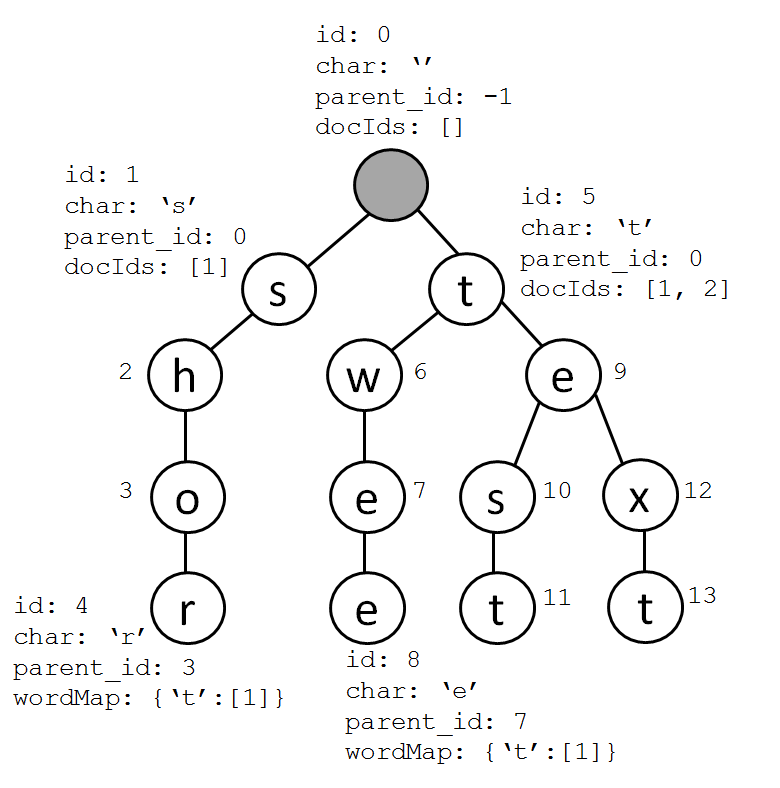
\includegraphics[scale=.35]{trie_maxdepth_figure}
  \caption{Structure of a trie index with a maximum depth of 4. If a word gets cut off by the depth limit, the substring remainder is stored at the leaves. Each substring remainder maps to a list of document ids with that remainder.}
\end{figure}

\subsection{Hybrid Tries}

\section{Performance and Comparison}

\subsection{Comparing Different Index Types}

\subsubsection{Index Creation}

\subsubsection{Index Lookups}


\begin{figure}[h!]
   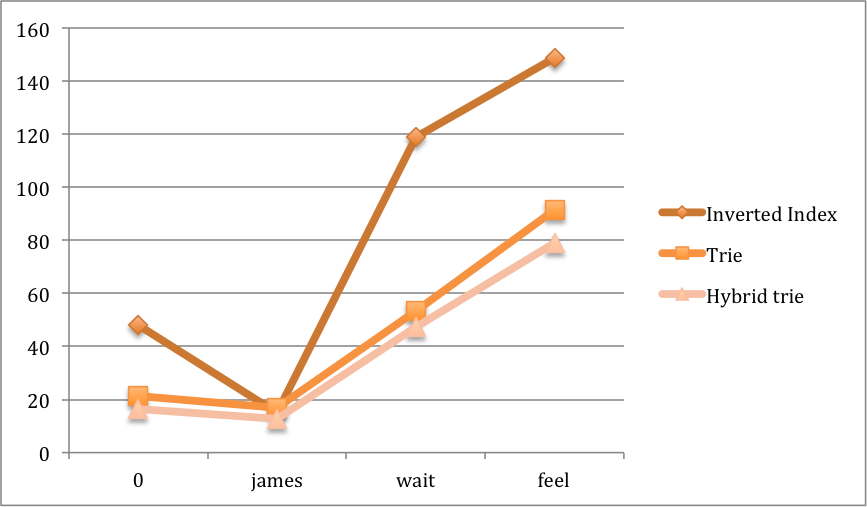
\includegraphics[scale=.53]{query-times}
  \caption{caption here}
\end{figure}

\subsection{Depth-Limiting for Tries}
As seen in Figure *****, the maximum depth parameter has an effect on lookup times in trie indexes. The graph shows the results for a trie index prefix search, but the similar results would be expected on suffix searches. A small set of input tweet data was used (367 KB data, about 2100 tweets), and the same three words were looked up in indexes created with differing max depths. The lookup time tends to decrease as the maximum depth increases; this is because depth cutoffs can result in slow searches through word mappings stored on leaf nodes (see section **** for details). The difference in times is more pronounced for the term ``feel'', with a drop from 26.78ms to 18.05ms. For the term ``james'', lookup times are much closer together and not as affected by depth limits. This is due to the fact that ``feel'' yielded many more results (85 results) than ``james'' (4 results), suggesting that more potential matches had to be searched at the leaf nodes for ``feel'' than for ``james''. Results for ``wait'' are between the others, and also show a moderate drop in lookup time as the maximum depth increases. This is most likely because ``wait'' produced a moderate 36 results, and therefore a moderate number of terms were searched at the leaves.

\begin{figure}[h!]
   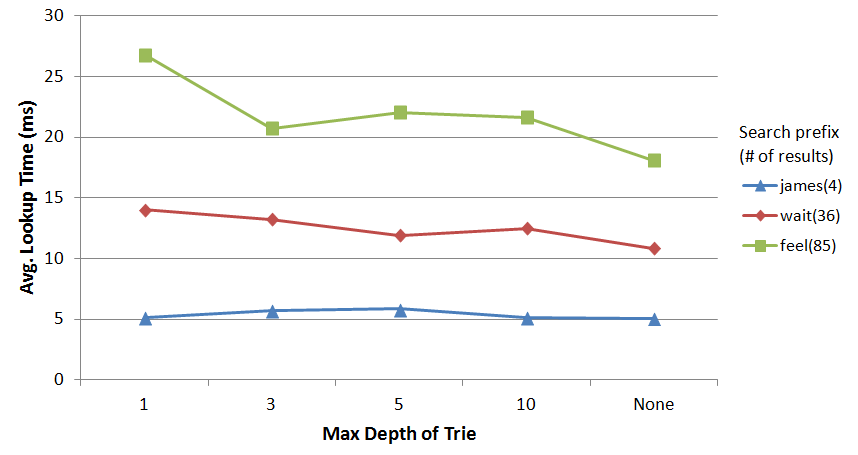
\includegraphics[scale=.43]{trie_maxdepth_graph}
  \caption{Maxiumum depth vs lookup times for a prefix trie index. A depth of ``None'' indicates that there is no limit. The results for three different search terms are shown. The dataset size was roughly 2100 tweets.}
\end{figure}

The data also shows that the number of results has an  impact on lookup time. The three graphs are tiered such that ``feel'', with the most results, is also the slowest query. While the lookup logic is parallelized so that the text for multiple matching document ids can be retrieved concurrently, the number of lookups that are done to retrieve this text has an impact on performance.




\section{Evaluation and Applications}

\subsection{Client-side vs. Server-side Search}




\begin{figure}[h!]
   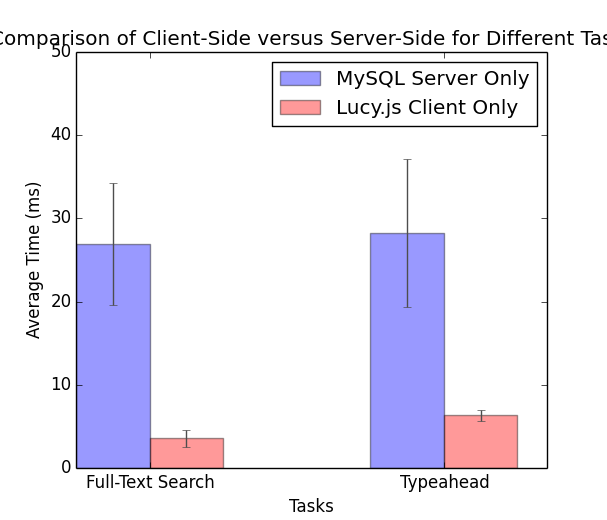
\includegraphics[scale=.53]{demo_results}
  \caption{caption here.}
\end{figure}



\section{Discussion}

\section{Future Work}

\section{Conclusion}

\bibliographystyle{abbrv}
\bibliography{paper}

\end{document}
